\documentclass{article}
\usepackage[utf8]{inputenc}
\usepackage[english]{babel}
 
\usepackage{hyperref}
\usepackage{graphicx}

\hypersetup{
    colorlinks=true,
    linkcolor=blue,
    filecolor=magenta,      
    urlcolor=cyan,
}
 
\urlstyle{same}

\title{Competitive programming website - CodeArea
        CSP[203]: Software System Laboratory}
\date{\today}

\begin{document}

\maketitle

\begin{table}[h!]
    \begin{center}
    \scalebox{1.2}{
    \begin{tabular}{c c}
         Authors & email id \\
         \hline
         Girish Kumar  & 2016csb1040@iitrpr.ac.in \\
         Karan Seghal & --change here--\\
         Chirag Khurana & --change here--\\
         Arunaksha Talukadar & --change here--
    \end{tabular}
    }
    \end{center}
\end{table}

\vspace{2cm}

\begin{figure}[h!]
    \centering
    
\includegraphics[width=0.4\linewidth]{rpr_logo.jpg}
\end{figure}


%----------------------------------------------------------
%                       Girish Kumar
%----------------------------------------------------------



\newpage

\section{Judge}

\subsection{introduction}
This is the important part of the CodeArea (competitive programming site name).
Main work of the judge is to execute user's codes and give them results of the execution e.g output for corresponding input or errors, compile time or run time errors. The judge take care of security and checks if the user program is not going to read or write other files on the server and executing other programs on the server.


\subsection{Supported languages}
In initial phase of the CodeArea we are supporting following programming languages:
\begin{enumerate}
    \item C
    \item C++14
    \item C++11
    \item JAVA 8
    \item Python 3.5
    \item Python 2.6
\end{enumerate}

\vspace{1cm}

\subsection{Facilities}
\vspace{0.3cm}
\subsubsection{Custom input-output}
To test the code we are providing custom input-output facility so user can test there code for corresponding input and output. Custom input-output will be implemented in the web-page using iframe.
\newpage
\subsubsection{Code Editor}
To make writing code easier, we are providing a code editor which can be implemented in the web-page using iframe. The editor provides basic functionalities of syntax highlighting, smart indenting, bracket completion, editor themes, fonts(small, medium, large).
All of these functionalities are powered by \href{https://ace.c9.io/}{ACE}, an open source library for code editor.
\begin{figure}[h!]
    \centering
    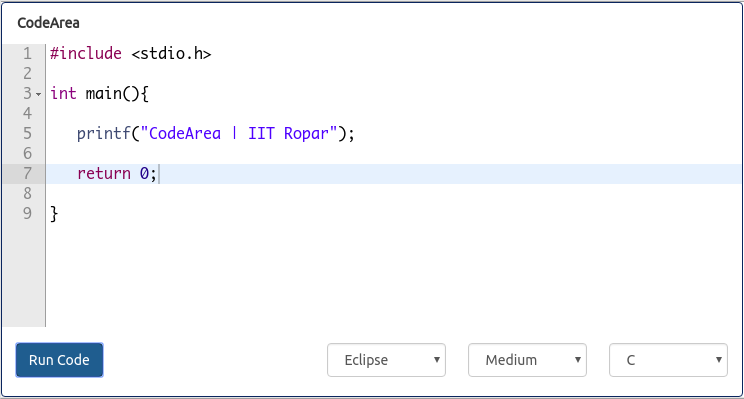
\includegraphics[width=0.8\linewidth]{sample_code_editor.png}
    \caption{ACE code editor}
    \label{fig:code_editor}
\end{figure}


\vspace{1.4cm}

\subsection{Submission}
On submission the language and the code is send to a python script which save the code to a temporary file with proper extension and we run the code on the server using os.system(command) and the program execution is killed if it takes more than the specified time. The output of the stdout and stderr is passed to a file and the content of the file is given to the user. Which contain errors in case of compile-time or run-time errors or output of program in case of successful completion of user program.
In case of submission against some test cases the content of the file is compared with right output for the problem.

\end{document}

%-----------------------------------------------------------
